\documentclass[journal]{IEEEtran}

\usepackage[utf8]{inputenc}
\usepackage[T1]{fontenc}
\usepackage{cite}
\usepackage{amsmath,amssymb,amsfonts}
\usepackage{algorithmic}
\usepackage{graphicx}
\usepackage{textcomp}
\usepackage{xcolor}

\begin{document}

\title{Clasificación de Texto con Naive Bayes Multinomial y Regresión Logística}

\author{Carlos Caicedo, Salomón Avila
\thanks{}}


\maketitle

\begin{abstract}
En este trabajo se aborda el problema de clasificación de texto utilizando un subconjunto de cuatro categorías del corpus \emph{20 Newsgroups} (\texttt{comp.graphics}, \texttt{sci.space}, \texttt{soc.religion.christian} y \texttt{talk.religion.misc}). Se entrenan y comparan un modelo Naive Bayes Multinomial y un modelo de Regresión Logística. Los resultados muestran que la Regresión Logística obtiene un mejor desempeño global (Accuracy = 0.892, F1 = 0.874) frente a Naive Bayes Multinomial (Accuracy = 0.802, F1 = 0.802), aunque este último resulta más simple y computacionalmente más económico. Se presentan matrices de confusión, curvas ROC y métricas de desempeño para ambos modelos.
\end{abstract}

\begin{IEEEkeywords}
Naive Bayes Multinomial, Regresión Logística, Clasificación de Texto, 20 Newsgroups
\end{IEEEkeywords}

\section{Introducción}
La clasificación de texto consiste en asignar automáticamente una categoría a un documento a partir de su contenido. Una de las representaciones más utilizadas para este propósito es la de bolsa de palabras (\emph{bag of words}), en la cual cada documento se representa mediante los conteos o las frecuencias de las palabras que lo componen.

El clasificador Naive Bayes Multinomial asume que las características se generan a partir de una distribución multinomial, la cual describe la probabilidad de observar determinados conteos entre un conjunto de categorías. Por esta razón, este modelo resulta apropiado cuando las características representan conteos de palabras o frecuencias dentro de los documentos.

En el presente laboratorio se compara el desempeño del Naive Bayes Multinomial frente a un modelo de Regresión Logística sobre un subconjunto de cuatro categorías del corpus 20 Newsgroups, con el fin de evaluar cuál de los dos enfoques ofrece un mejor equilibrio entre simplicidad y precisión en la tarea de clasificación de texto.

\section{Método}

\subsection{Conjunto de datos}
Se utilizó el corpus 20 Newsgroups, limitando el análisis a cuatro categorías para facilitar el estudio:

\begin{itemize}
    \item \texttt{comp.graphics}
    \item \texttt{sci.space}
    \item \texttt{soc.religion.christian}
    \item \texttt{talk.religion.misc}
\end{itemize}

Los conjuntos de entrenamiento y prueba se obtuvieron mediante la función \texttt{fetch\_20newsgroups}, especificando el parámetro \texttt{categories} con la lista anterior.

\subsection{Modelos}
Se entrenaron y compararon dos clasificadores sobre la representación de conteos de palabras de los documentos:

\begin{itemize}
    \item \textbf{Naive Bayes Multinomial}: modela la distribución de las características (conteos de palabras) mediante una distribución multinomial, asumiendo independencia condicional entre las características dado el conjunto de clases.
    \item \textbf{Regresión Logística}: modelo discriminativo lineal que estima directamente la probabilidad de pertenencia a cada clase a partir de las características de entrada, sin asumir una distribución generativa particular sobre los datos.
\end{itemize}

\subsection{Métricas de evaluación}
El desempeño de ambos modelos se evaluó mediante las métricas de \emph{Accuracy}, \emph{Precision}, \emph{Recall} y \emph{F1-score}, así como mediante la matriz de confusión y las curvas ROC (Receiver Operating Characteristic) por clase, calculadas bajo el esquema uno-contra-el-resto.

\section{Resultados}

\subsection{Métricas de desempeño}
La grafica \ref{fig:metrics_comparison} resume las métricas obtenidas por cada modelo sobre el conjunto de prueba.

\begin{figure}[!ht]
\centering
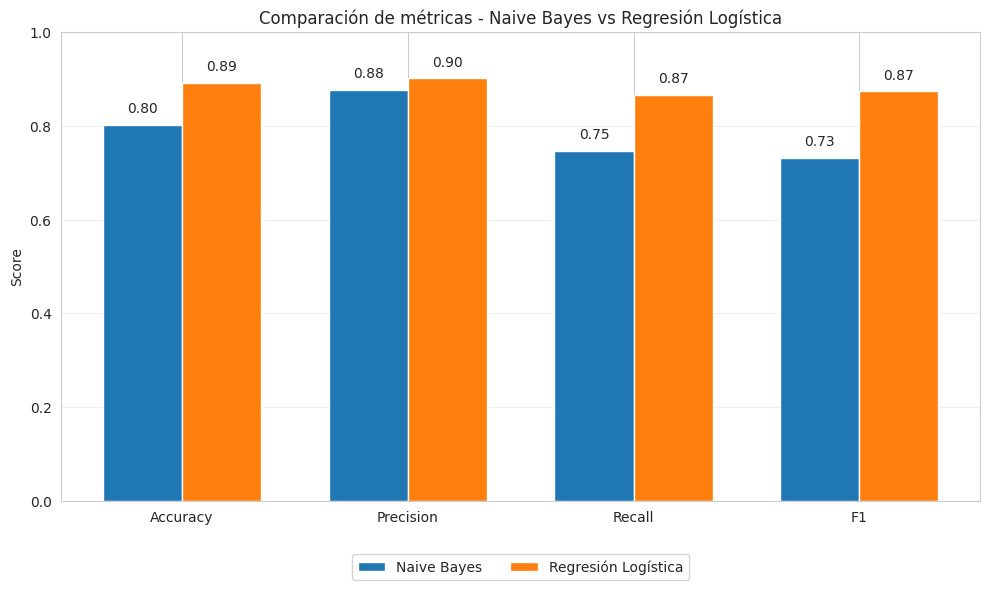
\includegraphics[width=\columnwidth]{metrics_comparison.png}
\caption{Comparación de las métricas Accuracy, Precision, Recall y F1-score entre Naive Bayes Multinomial (azul) y Regresión Logística (naranja).}
\label{fig:metrics_comparison}
\end{figure}

Como se observa en la gráfica \ref{fig:metrics_comparison}, la Regresión Logística supera a Naive Bayes Multinomial en las cuatro métricas evaluadas, con una mejora de aproximadamente 9 puntos porcentuales en Accuracy y de 7.2 puntos en F1-score.


\subsection{Matrices de confusión}
La Figura \ref{fig:confusion} presenta las matrices de confusión obtenidas para ambos modelos. En el caso de Naive Bayes Multinomial (izquierda), se observa una confusión considerable entre las clases \texttt{soc.religion.christian} y \texttt{talk.religion.misc}: 187 documentos de la clase \texttt{talk.religion.misc} fueron clasificados erróneamente como \texttt{soc.religion.christian}, lo que evidencia la dificultad del modelo para diferenciar estas dos clases con temáticas similares.

En contraste, la Regresión Logística (derecha) reduce notablemente esta confusión, clasificando correctamente 154 de los documentos de \texttt{talk.religion.misc} y disminuyendo a 60 los casos confundidos con \texttt{soc.religion.christian}. Las clases \texttt{comp.graphics} y \texttt{sci.space} presentan un desempeño alto en ambos modelos, aunque la Regresión Logística tiene un mayor número de errores dispersos entre clases (por ejemplo, 24 documentos de \texttt{comp.graphics} clasificados como \texttt{talk.religion.misc}).

\begin{figure}[!ht]
\centering
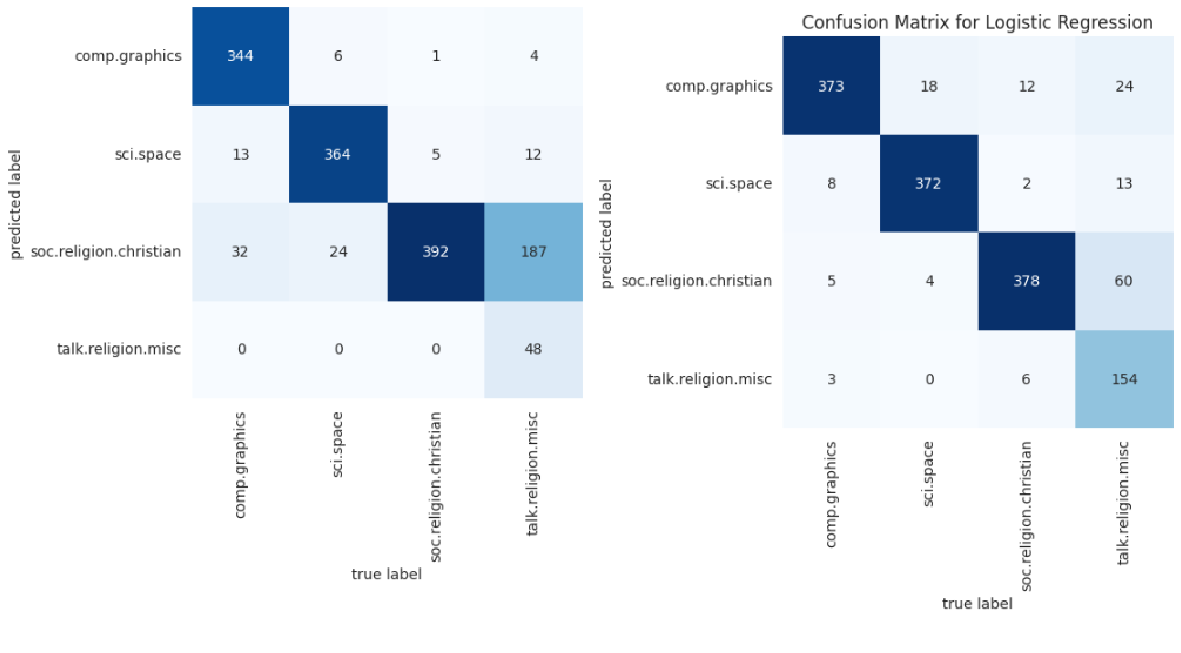
\includegraphics[width=\columnwidth]{confusion_matrices.png}
\caption{Matrices de confusión. Izquierda: Naive Bayes Multinomial. Derecha: Regresión Logística.}
\label{fig:confusion}
\end{figure}

\subsection{Curvas ROC}
Por último, la Figura \ref{fig:roc} muestra las curvas ROC por clase para ambos modelos, junto con el área bajo la curva (AUC) correspondiente. Para Naive Bayes Multinomial, las clases 0 y 1 (\texttt{comp.graphics} y \texttt{sci.space}) alcanzan valores de AUC de 0.990 y 0.993 respectivamente, mientras que la clase 3 (\texttt{talk.religion.misc}) obtiene el valor más bajo, con un AUC de 0.884, consistente con la mayor confusión observada para esta clase en la matriz de confusión.

En el caso de la Regresión Logística, se observa un comportamiento más equilibrado entre clases: la clase 3 mejora su AUC hasta 0.962, mientras que las clases 0 y 1 se mantienen en niveles similares (0.988 y 0.994). Esto confirma que, si bien ambos modelos distinguen adecuadamente entre las clases más diferentes, la Regresión Logística tiene un mejor equilibrio en la separación de las clases con temáticas similares.

\begin{figure}[!ht]
\centering
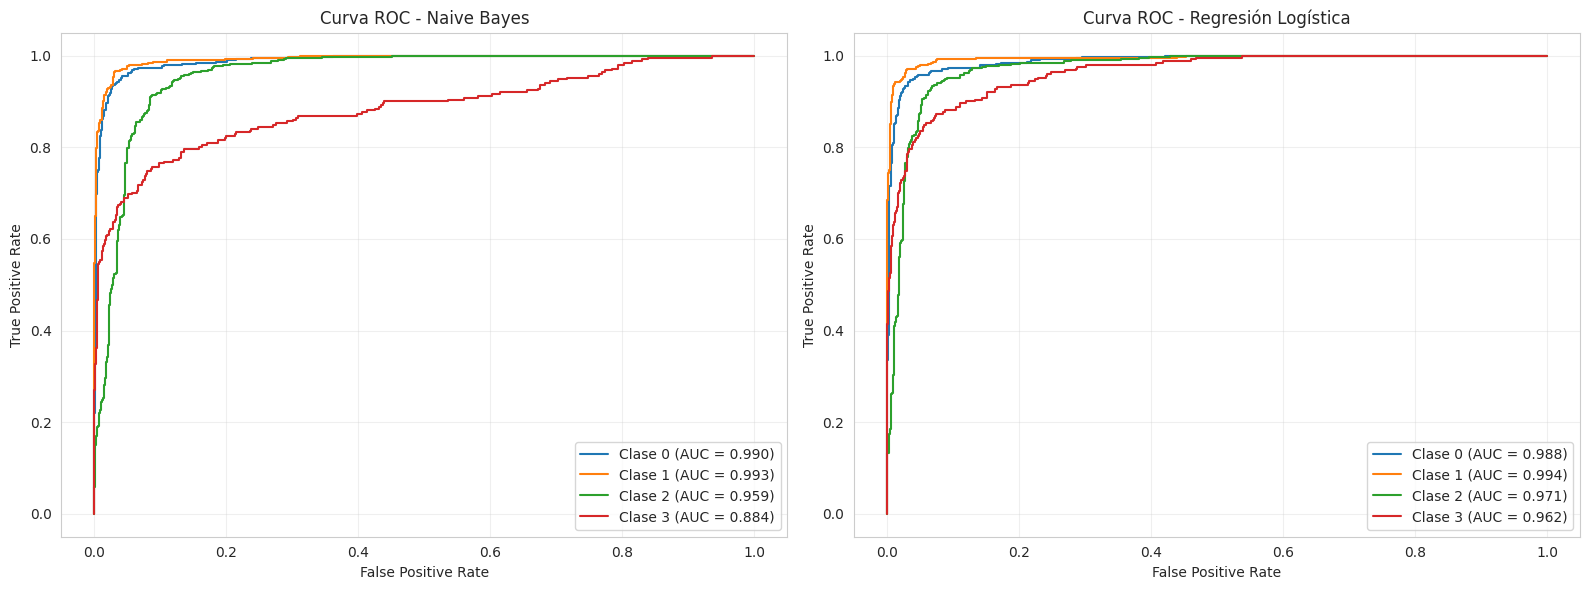
\includegraphics[width=\columnwidth]{roc_curves.png}
\caption{Curvas ROC por clase. Izquierda: Naive Bayes. Derecha: Regresión Logística. AUC indicado en la leyenda de cada clase.}
\label{fig:roc}
\end{figure}

\section{Conclusión}
Los resultados obtenidos muestran que, para la tarea de clasificación de texto sobre el subconjunto de cuatro categorías del corpus 20 Newsgroups, el modelo de Regresión Logística supera de manera consistente al Naive Bayes Multinomial en todas las métricas evaluadas (Accuracy, Precision, Recall y F1-score), así como en el área bajo la curva ROC para cada clase.

La principal fuente de error en ambos modelos se concentra en la distinción entre las clases \texttt{soc.religion.christian} y \texttt{talk.religion.misc}, dado el alto grado de similitud temático entre ellas. Sin embargo, la Regresión Logística logra reducir considerablemente este problema en comparación con Naive Bayes Multinomial.

A pesar de su menor desempeño, Naive Bayes Multinomial sigue siendo una alternativa útil cuando se requiere un modelo simple, interpretable y de bajo costo computacional, especialmente en escenarios con grandes volúmenes de datos o recursos limitados. La elección entre ambos modelos dependerá, del balance deseado entre precisión y simplicidad computacional.

\begin{thebibliography}{1}
\bibitem{b1} K. Lang, ``NewsWeeder: Learning to filter netnews,'' in \emph{Proceedings of the Twelfth International Conference on Machine Learning}, 1995, pp. 331--339.
\end{thebibliography}
 

\end{document}
